\documentclass[
12pt,						% Schriftgröße
DIV10,
german,						% für Umlaute etc
listof=totoc,				% Verzeichnisse im Inhaltsverzeichnis aufführen
bibliography=totoc, 		% Literaturverzeichnis im Inhaltsverzeichnis aufführen
index=totoc,				% Index im Inhaltsverzeichnis aufführen
oneside,
paper=a4,
headings=normal,
titlepage,					% es wird eine Titelseite verwendet
parskip=half,				% Abstand zwischen Absätzen (halbe Zeile)	
headsepline,        		% Linie unter Kopfzeile
final
]{scrbook} % alternativ: scrreprt, scrartcl


% Packages
% -----------------------------------
%Einstellungen der Seitenränder
\usepackage[inner=3.5cm,outer=2cm,top=2.5cm,bottom=2cm,includeheadfoot]{geometry}

%% Zitate
\usepackage{apacite} 					% Literatur-Referenzen: American Psycholog. Assoc.
\usepackage{natbib}						% definiert den Zitierstil als Autor (Jahr)
\usepackage{mdwlist}
\setcitestyle{round,aysep={}} 			% Indizierg. in runden Klammern, zw. Autor u. Jahr


%% Überschriften in Deutsch
% \usepackage[latin1]{inputenc} 		% Umlaute im Text
\usepackage[ansinew]{inputenc}        	% Umlaute ermöglichen - einkommentieren, falls oben nicht 															funktioniert
\usepackage[ngerman, english]{babel}   	% englische und deutsche Sprache, die letzte Sprache gibt an, in 													welcher Sprache die Überschriften (Literaturverzeichnis vs. 													References etc) angegeben werden
\usepackage[T1]{fontenc}
\hyphenation{voll-st\"andigen}

%%% Bilder
\usepackage{graphicx} 					% Grafiken einfügen (pdf,png - aber jpg vermeiden)
\graphicspath{{./Bilder/}}              % Pfad zu den Bildern
\usepackage{pdflscape}               	% Einzelne Seiten im Querformat möglich
\usepackage[pdftex]{xcolor}             % Eigene Farbdefinition möglich
\usepackage{subfigure}               	% für mehrere Grafinken in einer Figure
\usepackage{placeins}                	% Bessere Positionierung von Tabellen und Figures [\FloatBarrier]
\usepackage{float}						% Stellt die Platzierungsoption[H] zur Verfügung, mit der man flaots 												an die Stelle zwingen kann, wo sie definiert wurden.

%% für schöne Graphiken (können so direkt in Latex erstellt werden, sehr praktisch!)
\usepackage{tikz}
\usetikzlibrary{shapes.geometric}
\usetikzlibrary{shapes.arrows}
\usepackage{pgfplots}					% ermöglicht das Erstellen von Plots in der Tikzpicture-Umgebung
\usepackage{filecontents}				% ermöglicht das Einlesen der zu plottenden Daten aus .csv oder .txt-											  Datein

%%% Tabellen
\usepackage{longtable}               	% größere Tabellen mit Umbrüchen möglich 
\usepackage{ifthen}						% ermöglicht if-Abfragen
\usepackage{rotating}
\usepackage{array} 						% Für schönere und vielfältigere Tabellen
\usepackage{multirow} 					% Mehrere Spalten/Zeilen in einer Tabelle zusammenfassen 															(multicolumn, multirow}
\usepackage{booktabs}					% Das Paket stellt zwei Design-Paradigmen auf: 1. Vertikale Linien 													sind böse,  2. Doppelte Linien sind böse

% Ein paar Neudefinitionen zum Anpassen des multirow-Befehls an die booktabs-Umgebung
		\newcommand{\forloop}[5][1]{%
		\setcounter{#2}{#3}%
		\ifthenelse{#4}{#5\addtocounter{#2}{#1}%
		\forloop[#1]{#2}{\value{#2}}{#4}{#5}}%
		{}}
		\newcounter{crcounter}
		\newcommand{\compensaterule}[1]{%
		\forloop{crcounter}{1}{\value{crcounter} < #1}%
		{\vspace*{-\aboverulesep}\vspace*{-\belowrulesep}}}
		\newcommand{\multirowbt}[3]{\multirow{#1}{#2}%
		{\compensaterule{#1}#3}}
		
		\usepackage{epstopdf}
\usepackage{url}					  
\usepackage{tabularx} 				% bessere Gestaltung von Tabellen
\usepackage[active]{srcltx}
\usepackage{setspace} 				% Zeileneinstellung: 1,5-facher Zeilenabstand

%% Formeln
\usepackage{amsmath} 				% bessere Formelumgebung
\usepackage{amsfonts}               % Mehr Schriftarten in Formeln
\usepackage{amssymb}                % Sonderzeichen in Formeln
\usepackage{siunitx}				% ermöglicht Darstellung der Einheiten in SI Einheiten
\usepackage{textcomp}				% ermöglicht °C und € im Fließtext (mit \textcelsius) 

%% Verzeichnisse
\usepackage{nomencl}                % fürs Symbolverzeichnis	
\usepackage{booktabs}

%TODO
% Load the package
\usepackage{glossaries}
% Generate the glossary
\makeglossaries
%TODO end
\usepackage[ruled,vlined]{algorithm2e}
\newtheorem{mydef}{Merksatz}  		% Falls Beispiele, Merksätze m. fortl. Nr. gebr. werden
\newtheorem{bsp}{Beispiel}
\rmfamily 							% Serifenschrift
% \usepackage[margin=0.5in]{geometry}
\addtolength{\oddsidemargin}{.15in}
\addtolength{\evensidemargin}{-.15in}

\renewcommand{\familydefault}{\sfdefault}	
%\renewcommand{\familydefault}{\rmdefault}	

%% für Code im Anhang
\usepackage{listings} \lstset{numbers=left, numberstyle=\tiny, numbersep=5pt}
\lstset{language=Matlab,breaklines=true}
\usepackage{color}

\parindent0pt %Erstzeileneinzug abschalten


\newcounter{mytemp}
\newcounter{BlockCounter}
 \renewcommand{\theBlockCounter}{\Alph{BlockCounter}} 		% nummeriert Blöcke in Flowcharts mit A,B,C statt 1,2,3
 
 \addtocounter{secnumdepth}{1}
\addtocounter{tocdepth}{1}

% Alle Querverweise und URLs als Link darstellen
% In der PDF-Ausgabe
\usepackage[colorlinks=true, bookmarks, bookmarksnumbered, bookmarksopen, bookmarksopenlevel=1,
linkcolor=black, citecolor=black, urlcolor=black, filecolor=black,
pdfpagelayout=OneColumn, pdfnewwindow=true,
pdfstartview=Fit, plainpages=false, pdfpagelabels, pdftex,
pdfauthor={Vorname Nachname},
pdftitle={Titel der Arbeit},
pdfsubject={Masterarbeit},
pdfkeywords={Keyword1, Keyword2, Keyword3, ...}]{hyperref}

% Farben und Logos siehe: https://intranet.avt.rwth-aachen.de/Intranet/AVT/wiki/index.php/Logos#Farben  
	% Farbennamen und -definitionen sind an die AVT-Powerpointpräsentation angelehnt. 
%	\definecolor{avtcolor}{rgb}{0,0.537,0.820}	% Mit "rgb" muss man von den Angaben aus Word (= denen von der Webseite) immer Umrechnen
%	\definecolor{avtcolor}{RGB}{14,133,196}			% mit "RGB" (großgeschrieben) muss man nicht Umrechen!
%	\definecolor{rwthblue}{RGB}{0,83,159}
%	\definecolor{186blau}{rgb}{0.729 ,0.859, 0.941} % ganz helles blau
%	\definecolor{135blau}{rgb}{0.529,0.82,0.941} % auch ganu helles Blau
%	\definecolor{64blau}{rgb}{0.25,0.741,0.827} % mittelblau (Logo 2. Klötzchen von links)
%	\definecolor{79gruen}{rgb}{0.31,0.663,0.153} % dunkelgrün aus dem Logo
%	\definecolor{194gruen}{rgb}{0.761,0.81,0} % hellgrün
%	\definecolor{178grau}{rgb}{0.7,0.7, 0.7}
%	\definecolor{0blau}{rgb}{0 ,0.506, 0.776} % farblich gleich mit AVTcolor, dunkelblau aus Logo
%	%	
	
	%% LTT-Farben
	% Hausfarbe RWTH blau
	\definecolor{rwthblue100}{RGB}{0,84,159}
	\definecolor{rwthblue75}{RGB}{64,127,183}
	\definecolor{rwthblue50}{RGB}{142,186,229}
	\definecolor{rwthblue25}{RGB}{199,221,242}
	\definecolor{rwthblue10}{RGB}{232,241,250}
	
	% schwarz
	\definecolor{black100}{RGB}{0,0,0}
	\definecolor{black75}{RGB}{100,101,103}
	\definecolor{black50}{RGB}{156,158,159}
	\definecolor{black25}{RGB}{207,209,210}
	\definecolor{black10}{RGB}{236,237,237}
	
	% magenta
	\definecolor{magenta100}{RGB}{227,0,102}
	\definecolor{magenta75}{RGB}{233,96,136}
	\definecolor{magenta50}{RGB}{241,158,177}
	\definecolor{magenta25}{RGB}{249,210,218}
	\definecolor{magenta10}{RGB}{253,238,240}
	
	% gelb
	\definecolor{yellow100}{RGB}{255,237,0}
	\definecolor{yellow75}{RGB}{255,240,85}
	\definecolor{yellow50}{RGB}{255,245,155}
	\definecolor{yellow25}{RGB}{255,250,209}
	\definecolor{yellow10}{RGB}{255,253,238}
	
	% petrol
	\definecolor{petrol100}{RGB}{0,97,101}
	\definecolor{petrol75}{RGB}{45,127,131}
	\definecolor{petrol50}{RGB}{125,164,167}
	\definecolor{petrol25}{RGB}{191,208,209}
	\definecolor{petrol10}{RGB}{230,236,236}
	
	% türkis
	\definecolor{cyan100}{RGB}{0,152,161}
	\definecolor{cyan75}{RGB}{0,177,183}
	\definecolor{cyan50}{RGB}{137,204,207}
	\definecolor{cyan25}{RGB}{202,231,231}
	\definecolor{cyan10}{RGB}{235,246,246}
	
	% grün
	\definecolor{green100}{RGB}{87,171,39}
	\definecolor{green75}{RGB}{141,192,96}
	\definecolor{green50}{RGB}{184,214,152}
	\definecolor{green25}{RGB}{221,235,206}
	\definecolor{green10}{RGB}{242,247,236}
	
	% maigrün
	\definecolor{maygreen100}{RGB}{189,205,0}
	\definecolor{maygreen75}{RGB}{208,217,92}
	\definecolor{maygreen50}{RGB}{224,230,154}
	\definecolor{maygreen25}{RGB}{240,243,208}
	\definecolor{maygreen10}{RGB}{249,250,237}
	
	% orange
	\definecolor{orange100}{RGB}{246,168,0}
	\definecolor{orange75}{RGB}{250,190,80}
	\definecolor{orange50}{RGB}{253,212,143}
	\definecolor{orange25}{RGB}{254,234,201}
	\definecolor{orange10}{RGB}{255,247,234}
	
	% Rot
	\definecolor{red100}{RGB}{204,7,30}
	\definecolor{red75}{RGB}{216,92,65}
	\definecolor{red50}{RGB}{230,150,121}
	\definecolor{red25}{RGB}{243,205,187}
	\definecolor{red10}{RGB}{250,235,227}
	
	% bordeaux
	\definecolor{darkred100}{RGB}{161,16,53}
	\definecolor{darkred75}{RGB}{182,82,86}
	\definecolor{darkred50}{RGB}{205,139,135}
	\definecolor{darkred25}{RGB}{229,197,192}
	\definecolor{darkred10}{RGB}{245,232,229}
	
	% Violett
	\definecolor{violet100}{RGB}{97,33,88}
	\definecolor{violet75}{RGB}{131,78,117}
	\definecolor{violet50}{RGB}{168,133,158}
	\definecolor{violet25}{RGB}{210,192,205}
	\definecolor{violet10}{RGB}{237,229,234}
	
	% Lila
	\definecolor{purple100}{RGB}{122,111,172}
	\definecolor{purple75}{RGB}{155,145,193}
	\definecolor{purple50}{RGB}{188,181,215}
	\definecolor{purple25}{RGB}{222,218,235}
	\definecolor{purple10}{RGB}{242,240,247}
	
	% durch Definitionen in Tikz-Option kann der Plot in RWTH-Farben dargestellt werden.
	% zB \draw[color=rwthblue100] (0,0)-- (2,2) macht eine diagonale Linie in dunkelblau

% Chemische Formeln
\usepackage[version=4]{mhchem}	% Für die Darstellung chemischer Formeln (muss leider entweder von Hand eingebunden werden (Adminrechte nötig)  oder das mhchem.sty-file muss in dem selben Ordner wie das LaTeX-file liegen, damit LaTeX es finden kann.
\usepackage{chemfig} % Für Strukturformeln und ähnliches

%Zusätzliche Packages tima01
\usepackage{todonotes} %hiermit kann man todos einfügen ist ganz nett z.B. an Stellen wo später Bilder hin sollen
%\usepackage[decimalsymbol=comma,digitsep=period]{siunitx}   % Nutzen von Einheiten!
%\usepackage{eurosym} % hiedrin stehen alle Voreinstellungen

\DeclareSIUnit{\EUR}{\text{\euro}}
\newcommand{\abs}[1]{\ensuremath{\left\vert#1\right\vert}} %Betragsfunktion

\makenomenclature

\begin{document}

% Einrücken von Absätzen verhindern und 1.5 Zeilen Absatzabstand
\setlength{\parindent}{0pt}
\setlength{\parskip}{1.5ex plus0.5ex minus0.5ex}

\pagenumbering{roman} % Die ersten Seiten werden römisch nummeriert
  
  \numberwithin{equation}{chapter} %Gleichungen sollen mit Kapitelnummer nummeriert werden (z.Bsp. 4.1)
  \numberwithin{table}{chapter} %Tabellen sollen mit Kapitelnummer nummeriert werden (z.Bsp. 4.1)
  \numberwithin{figure}{chapter} %Abb. sollen mit Kapitelnummer nummeriert werden (z.Bsp. 4.1)

  \onehalfspacing		% 1,5facher Zeilenabstand
  \pagestyle{headings}	

  % Deckblatt des Dokuments 

%% das hier einkommentieren, wenn nicht das RWTH-Logo genutzt wird
%\thispagestyle{empty}
%\begin{titlepage}
%\vspace*{-2cm}
%\begin{figure*}
%\vspace*{-1.7cm}
%\raisebox{-3,5mm}
%{
\includegraphics[width=1.0\textwidth]{./Bilder/avt}}
%\end{figure*}

%% das hier einkommentieren, wenn das Corporate Design verwendet wird

%Einf�gen des Institutskopf
\thispagestyle{empty}
\begin{titlepage}
\vspace*{-3cm}
\hfill 
%\raisebox{-7,5mm}
{
\includegraphics[width=12cm]{./grafiken/rwth_ltt_en_rgb.png}} % hier nach Bedarf das deutsche Logo einbinden
%\vspace*{-0.5cm}

%\begin{picture}(0,0)
%\raisebox{3mm}{\line(0,0){0}}
%\end{picture}

\begin{minipage}[t]{16cm}
\begin{flushleft}
%\normalsize{\textbf{Diese Arbeit wurde vorgelegt am Lehrstuhl f�r Systemverfahrenstechnik} \newline 
%The present work was submitted to Chair of Process Systems Engineering}\\ %Institut eintragen!
\normalsize{\textbf{The present work was submitted to Chair of Technical Thermodynamics}}\\
\end{flushleft}
\end{minipage}
\vspace{2.5cm}
% Ende Instituskopf

\begin{center}
\begin{LARGE}
Enter a fancy title\\ % Titel eintragen
\end{LARGE}
\vspace{1cm}
\large{Bachelor-/ Masterthesis} % Art der Arbeit eintragen
\end{center}
% Beginn Titelseite
\begin{flushleft}

\vspace{2cm}
%\normalsize{vorgelegt von}\\
%\normalsize{\textbf{Nachname, Vorname}}\\
%\normalsize{Matrikelnummer xxx xxx}\\
%\normalsize{Bachelor-, Master-, Diplom-, Magisterarbeit}\\
%\vspace{2.5cm}
\normalsize{presented by}\\ % nach Bedarf die deutsche Version einkommentieren
\normalsize{\textbf{Nachname, Vorname}}\\ % Name eintragen
\normalsize{StudentID no. xxx xxx}\\ % Matrikelnummer eintragen
\vspace{2cm}
\normalsize{\textbf{Supervisor:}}\\	%richtigen Erstpr�fer eintragen
\normalsize{Vorname Nachname, M.Sc.}\\		%richtigen Zweitpr�fer eintragen

\vspace{2cm}
\normalsize{$1^{st}$ Examiner: Univ.-Prof. Dr.-Ing. Andr� Bardow}\\	%richtigen Erstpr�fer eintragen (evt ins Deutsche �bersetzen)
\normalsize{$2^{nd}$ Examiner: Jun.-Prof. Dr. Kai Leonhard}\\		%richtigen Zweitpr�fer eintragen
\end{flushleft}
\vfill

\begin{flushright}
\normalsize{Aachen, September 30, 2016} %VORSICHT: \today-Befehl gibt aktuelles Datum (z.B. "10. Juli 2015", bei Einstellung auf englisch "July 10, 2015") aus ggf. in Abgabedatum �ndern!
\end{flushright}

\end{titlepage}

\thispagestyle{empty}
\cleardoublepage % ensprechende Einträge überarbeiten
  \addcontentsline{toc}{chapter}{Abstract}
% Abstract
{\large \textbf{\textsf{Abstract}}}
\vspace*{3em}

bli bla blubb








\cleardoublepage
 % ensprechende Einträge überarbeiten
  
% nachfolgend auskommentiertes ist kein schöner Stil, lieber bei \usepackage{babel} Englisch auswählen  
% \renewcommand*\contentsname{Table of contents}
  \tableofcontents					% Inhaltsverzeichnis einfügen
  \setlength{\nomlabelwidth}{3cm}
%\renewcommand*\listfigurename{List of figures}
  \listoffigures				  % Abbildungsverzeichnis einfügen
% \renewcommand*\listtablename{List of tables}
  \listoftables						% Tabellenverzeichnis einfügen

  \thispagestyle{empty}   % Erzwungener Seitenumbruch
  \cleardoublepage        %  

  \pagenumbering{arabic}  % Ab hier Seitennummern mit arabischen Zahlen
  \setcounter{page}{1}    % Nummerierung beginnt bei 1


% +++++++++ ab hier jetzt die eigentlichen Dokumente einzufügen. Jeweils mit \include{...}.  ++++++++++++%
  \chapter{Introduction}
Lorem ipsum dolor sit amet, consectetuer adipiscing elit, sed diam nonummy nibh euismod tincidunt ut laoreet dolore magna aliquam erat volutpat. Ut wisi enim ad minim veniam, quis nostrud exerci tation ullamcorper suscipit lobortis nisl ut aliquip ex ea commodo consequat. Duis autem vel eum iriure dolor in hendrerit in vulputate velit esse molestie consequat, vel illum dolore eu feugiat nulla facilisis at vero et accumsan et iusto odio dignissim qui blandit praesent luptatum zzril delenit augue duis dolore te feugait nulla facilisi. Lorem ipsum dolor sit amet, consectetuer adipiscing elit, sed diam nonummy nibh euismod tincidunt ut laoreet dolore magna aliquam erat volutpat. Ut wisi enim ad minim veniam, quis nostrud exerci tation ullamcorper suscipit lobortis nisl ut aliquip ex ea commodo consequat. Duis autem vel eum iriure \SI{23}{\watt\per\square\meter}dolor in hendrerit in vulputate velit esse molestie consequat, vel illum dolore eu feugiat nulla facilisis at vero et accumsan et iusto odio dignissim qui blandit praesent luptatum zzril delenit augue duis dolore te feugait nulla facilisi. Nam liber tempor cum soluta nobis eleifend option congue nihil imperdiet doming id quod mazim placerat facer possim assum.

\begin{equation}
\dot{Q}=\dot{m}\cdot c_p \cdot \Delta \vartheta
\end{equation}

Lorem ipsum dolor sit amet, consectetuer adipiscing elit, sed diam nonummy nibh euismod tincidunt ut laoreet dolore magna aliquam erat volutpat. Ut wisi enim ad minim veniam, quis nostrud exerci tation ullamcorper suscipit lobortis nisl ut aliquip ex ea commodo consequat. Duis autem vel eum iriure dolor in hendrerit in vulputate velit esse molestie consequat, vel illum dolore eu feugiat nulla facilisis at vero et accumsan et iusto odio dignissim qui blandit praesent luptatum zzril delenit augue duis dolore te feugait nulla facilisi (Tabelle \ref{tab:Tabelle}). Lorem ipsum dolor sit amet, consectetuer adipiscing elit, sed diam nonummy nibh euismod tincidunt ut laoreet dolore magna aliquam erat volutpat.Ut wisi enim ad minim veniam, quis nostrud exerci tation ullamcorper suscipit lobortis nisl ut aliquip ex ea commodo consequat. Duis autem vel eum iriure dolor in hendrerit in vulputate velit esse molestie consequat, vel illum dolore eu feugiat nulla facilisis at vero et accumsan et iusto odio dignissim qui blandit praesent luptatum zzril delenit augue duis dolore te feugait nulla facilisi. Nam liber tempor cum soluta nobis eleifend option congue nihil imperdiet doming id quod mazim placerat facer possim assum. Ut wisi enim ad minim veniam, quis nostrud exerci tation ullamcorper suscipit lobortis nisl ut aliquip ex ea commodo consequat. Duis autem vel eum iriure dolor in hendrerit in vulputate velit esse molestie consequat, vel illum dolore eu feugiat nulla facilisis at vero et accumsan et iusto odio dignissim qui blandit praesent luptatum zzril delenit augue duis dolore te feugait nulla facilisi. Nam liber tempor cum soluta nobis eleifend option congue nihil imperdiet doming id quod mazim placerat facer possim assum.

\begin{table}[htb]
	\caption{Das ist eine Testtabelle}\vspace{6pt}
	\centering
\begin{tabular}{cr} 
\toprule
\textbf{Überschrift links} & \textbf{Überschrift rechts}\\
\midrule 
links oben & rechts oben \\  
links unten & rechts unten \\ 
\bottomrule 
\end{tabular}
\label{tab:Tabelle}
\end{table}



Lorem ipsum dolor sit amet, consectetuer adipiscing elit, sed diam nonummy nibh euismod tincidunt ut laoreet dolore magna aliquam erat volutpat. Ut wisi enim ad minim veniam, quis nostrud exerci tation ullamcorper suscipit lobortis nisl ut aliquip ex ea commodo consequat. Duis autem vel eum iriure dolor in hendrerit in vulputate velit esse molestie consequat, vel illum dolore eu feugiat nulla facilisis at vero et accumsan et iusto odio dignissim qui blandit praesent luptatum zzril delenit augue duis dolore te feugait nulla facilisi (Tabelle \ref{fig:PCM_Slurry1}). Lorem ipsum dolor sit amet, consectetuer adipiscing elit, sed diam nonummy nibh euismod tincidunt ut laoreet dolore magna aliquam erat volutpat. Ut wisi enim ad minim veniam, quis nostrud exerci tation ullamcorper suscipit lobortis nisl ut aliquip ex ea commodo consequat. Duis autem vel eum iriure dolor in hendrerit in vulputate velit esse molestie consequat, vel illum dolore eu feugiat nulla facilisis at vero et accumsan et iusto odio dignissim qui blandit praesent luptatum zzril delenit augue duis dolore te feugait nulla facilisi. Nam liber tempor cum soluta nobis eleifend option congue nihil imperdiet doming id quod mazim placerat facer possim assum (siehe dazu \cite{lanzerath2013modellgestuetzteentwicklungvon}).

\begin{figure}[htb]
	\centering
		\hfill
		\subfigure[Isosterendiagramm]{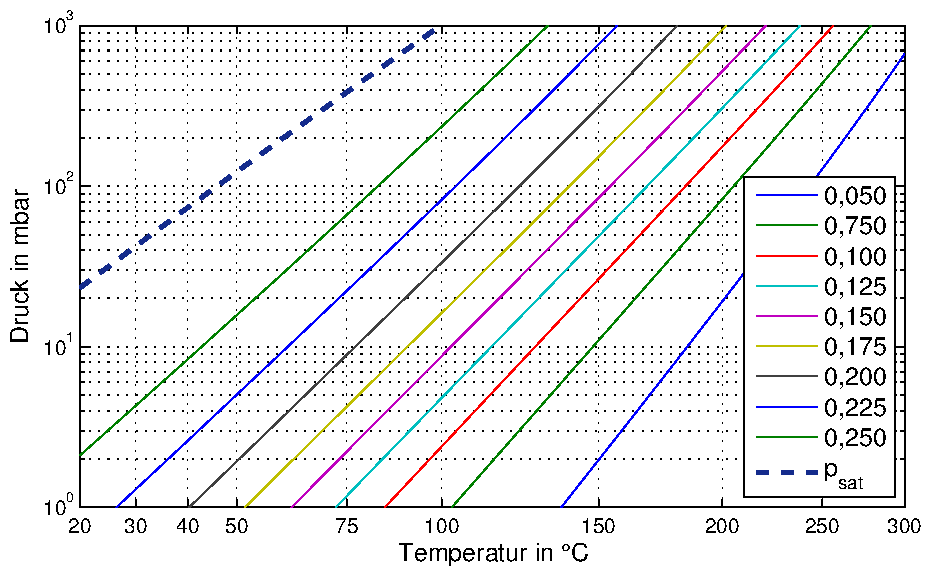
\includegraphics[width=0.45\textwidth]{grafiken/IsostereNunez-eps-converted-to.pdf}}
		\hfill
		\subfigure[Idealer Zyklus]{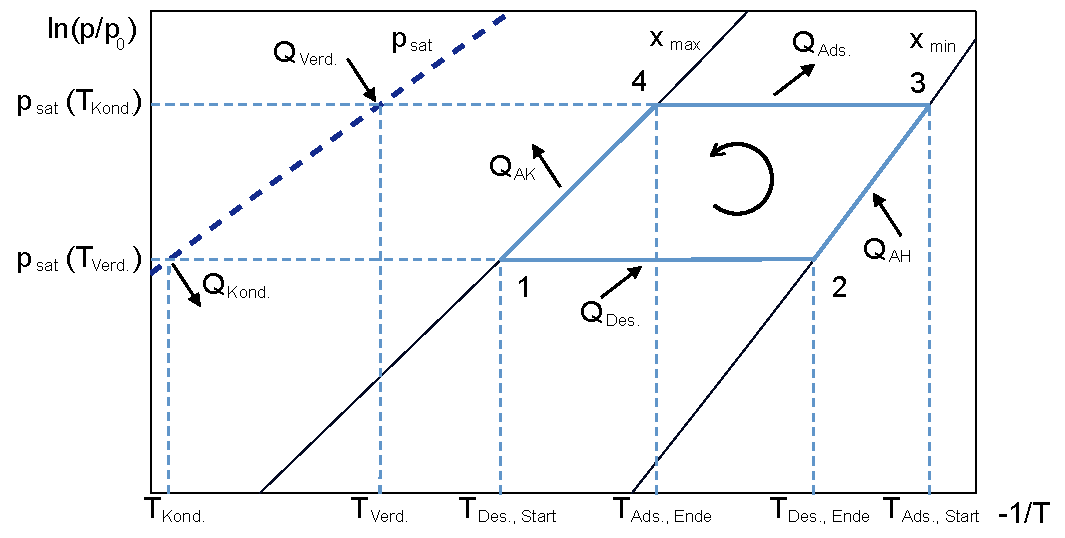
\includegraphics[width=0.45\textwidth]{grafiken/zyklus_schema_alt.pdf}}
		\hfill~
	\caption{Zyklus und Isosterendiagramm}
	\label{fig:PCM_Slurry1}
\end{figure}

Lorem ipsum dolor sit amet, consectetuer adipiscing elit, sed diam nonummy nibh euismod tincidunt ut laoreet dolore magna aliquam erat volutpat. Ut wisi enim ad minim veniam, quis nostrud exerci tation ullamcorper suscipit lobortis nisl ut aliquip ex ea commodo consequat. Duis autem vel eum iriure dolor in hendrerit in vulputate velit esse molestie consequat, vel illum dolore eu feugiat nulla facilisis at vero et accumsan et iusto odio dignissim qui blandit praesent luptatum zzril delenit augue duis dolore te feugait nulla facilisi (Tabelle \ref{fig:PCM_Slurry1}). Lorem ipsum dolor sit amet, consectetuer adipiscing elit, sed diam nonummy nibh euismod tincidunt ut laoreet dolore magna aliquam erat volutpat. Ut wisi enim ad minim veniam, quis nostrud exerci tation ullamcorper suscipit lobortis nisl ut aliquip ex ea commodo consequat. Duis autem vel eum iriure dolor in hendrerit in vulputate velit esse molestie consequat, vel illum dolore eu feugiat nulla facilisis at vero et accumsan et iusto odio dignissim qui blandit praesent luptatum zzril delenit augue duis dolore te feugait nulla facilisi. Nam liber tempor cum soluta nobis eleifend option congue nihil imperdiet doming id quod mazim placerat facer possim assum.

% bestimmte Shapes vordefinieren
\tikzstyle{block} = [rectangle, draw=black, fill=blue!0, 
    text width=6cm, text centered, rounded corners, node distance=2cm, minimum width=4cm, minimum height=0.5cm]
    
\tikzstyle{cloud} = [draw, ellipse,fill=red!0, node distance=3cm, minimum height=2em]

% die Tikz-Umgebung für das Bild anlegen    
\begin{tikzpicture}
\label{fig:algorithm}
    % Place nodes

   \node[cloud] (start) {START};
   
  \node [block, right of=start,xshift = 3.5cm] (start2) {\textbf{Initialisation}};
   
 
  % Draw edges
  \draw (start) -- (start2);

\end{tikzpicture}
%  \include{chapters/kapitel1}
%  \include{chapters/kapitel2} etc


% Literaturverzeichnis -----------------------------------------------------
%		Das Literaturverzeichnis wird aus der Datenbank Bibliographie.bib 
% 	erstellt. Die genaue Verwendung von bibtex wird hier jedoch nicht erklärt.
%		Link: http://de.wikipedia.org/wiki/BibTeX
% --------------------------------------------------------------------------
%\nocite{*}											% Einbinden aller Quellen (auch der nciht zitierten) aus dem nachfolgenden Dokument
%\renewcommand*{\bibname}{References}
\bibliography{literature/thesis_lit}		    % Einbinden der Datei literatur.bib
\bibliographystyle{apacite} 	% DIN-Stil des Literaturverzeichnisses

%\DefineBibliographyStrings{german}{%
%phdthesis ={Dissertation}
%}
%\bibliographystyle{gerunsrt}


% ++++++++++++++++++++ ANHANG +++++++++++++++++++++++++++++++++++++++++++++++++++++++++++++++++++
\appendix %hier beginnt der Anhang
  
    \makenomenclature %Nomenklatur wird erstellt, aber noch nicht ausgegeben


\renewcommand{\nomname}{List of Abbreviations and Symbols Used} % Deutsche �berschrift evt einf�gen
\newcommand{\einheit}[1]{\renewcommand{\nomentryend}{\hfill $\left[ #1 \right]$} } % Einheiten k�nnen angegeben werden 

% ++++ Damit Nomenklatur im Anhang als eigenes Chapter aufgef�hrt wird 
\setlength{\nomlabelwidth}{20mm}  % LabelBreite
\makeatletter   
\renewcommand{\thenomenclature}{%
\chapter{\nomname}
\list{}{
\labelwidth\nom@tempdim
\leftmargin\labelwidth
\advance\leftmargin\labelsep
\let\makelabel\nomlabel
}
}
\makeatother
% ++++ Ende eigenes Chapter

% ++++ Die einzelnen Teile der Nomenklatur werden definiert ++++
\renewcommand{\nomgroup}[1]{%
	\ifthenelse{\equal{#1}{S}}{\item[\textbf{List of Symbols}]}{%
		\ifthenelse{\equal{#1}{A}}{\item[\textbf{List of Abbreviations}]} {
		  \ifthenelse{\equal{#1}{I}}{\item[\textbf{List of indices}]} {} } }	
		 }

% +++++++  Ab hier die Nomenklatureintr�ge bearbeiten ++++++++++++

% VERZEICHNIS DER FORMELZEICHEN
\nomenclature[S]{$\varphi$}{smoothed switching function between 0 and $\Delta h_i$ \einheit{-}}


% VERZEICHNIS DER ABK�RZUNGEN
 \nomenclature[A]{$DAE$}{Differential-algebraische Gleichung}%


% VERZEICHNIS DER INDIZES
\nomenclature[I]{$UBD$}{upper bounding}%


    % genauso wie im Hauptteil  
    \printnomenclature % Ausgabe der Nomenklatur
    
    % falls das Formelverzeichnis nicht kompiliert, müssen evt. die Editoreinstellungen geändert werden. Dazu unter Optionen - Texmaker konfigurieren - MakeIndex den Text makeindex %.idx durch makeindex.exe %.nlo -s nomencl.ist -o %.nl ersetzen
    
% +++++++ hier können noch weitere Datein als Anhang eingebunden werden ++++++++
%\include{AppA}
%\include{AppB}
% auch hier können wieder Chapter z.Bsp. mit Modellgleichungen eingebunden werden
%
%tima01 hier wird jetzt Liste eingeblendet mit Todo´s die abgearbeitet werden müssen
%\listoftodos %TODOs

\end{document}